% !TEX program = xelatex

\documentclass[crop,tikz]{standalone}

\usepackage{amsmath}
\usepackage{fontspec}
\setmainfont{CMU Serif}

\usepackage{pgfplots}
\usepgfplotslibrary{fillbetween}

\usetikzlibrary{arrows.meta}
\usetikzlibrary{calc,patterns,angles,quotes}

\pgfdeclarelayer{background}
\pgfdeclarelayer{foreground}
\pgfsetlayers{background,foreground}

\pgfdeclarepatternformonly{my crosshatch dots}{\pgfqpoint{-2pt}{-1pt}}{\pgfqpoint{5pt}{5pt}}{\pgfqpoint{11pt}{10pt}}%
{
  \pgfpathcircle{\pgfqpoint{-1pt}{0pt}}{.5pt}
  \pgfpathcircle{\pgfqpoint{4pt}{3pt}}{.5pt}
  \pgfusepath{fill}
}

\tikzset{%
  dots/.style={%
    line cap=round,
    dash pattern=on 0 off 1cm/32
  }
}

\tikzset{
  boat/.pic={
    code={
      % Hull
      \coordinate (bow) at (0,0);
      \coordinate (stern) at (4,-1.25);

      \coordinate (stern_left_top) at ($ (stern) + (-0.75,-0.25) $);
      \coordinate (stern_left_bottom) at ($ (stern_left_top) + (0,-0.5) $);
      \coordinate (stern_right_top) at ($ (stern) + (0.75,0.25) $);
      \coordinate (stern_right_bottom) at ($ (stern_right_top) + (0,-0.5) $);

      % \draw[gray,dotted] (bow) -- (stern);
      \draw[fill=white]
        (stern_left_top)
        --
        (stern_right_top)
        --
        (stern_right_bottom)
        to[out=-125,in=-15,looseness=0.8]
        (stern_left_bottom)
        --
        (stern_left_top);

      \draw[fill=white]
        (bow)
        to[out=-45,in=-190,looseness=0.8]
        (stern_left_top)
        --
        (stern_left_bottom)
        to[out=-190,in=-75,looseness=0.8]
        (bow);
        
      \draw[fill=white]
        (bow)
        to[out=-45,in=-190,looseness=0.8]
        (stern_left_top)
        --
        (stern_right_top)
        to[out=160,in=0,looseness=0.5]
        (bow);
      
      \draw[fill=white]
        ($ (stern_left_top) + (0,0.05) $)
        --
        ($ (stern_right_top) + (-0.15,0) $)
        to[out=160,in=-10,looseness=0.4]
        ($ (stern_right_top) + (-2.45,0.6) $)
        --
        ($ (stern_left_top) + (-2.15,0.8) $)
        to[out=-35,in=-190,looseness=0.6]
        ($ (stern_left_top) + (0,0.05) $);
      % \draw ($ (stern_right_top) + (-2.45,0.6) $) -- ($ (stern_right_top) + (-2.45,0) $);

      % Mast
      \coordinate (mast_bottom) at ($ (bow)!0.4!(stern) $);
      \coordinate (mast_bottom_left) at ($ (mast_bottom) + (-0.05,0.03) $);
      \coordinate (mast_bottom_right) at ($ (mast_bottom) + (0.05,-0.03) $);
      \coordinate (mast_top) at ($ (mast_bottom) + (0,3.5) $);
      \coordinate (mast_top_left) at ($ (mast_top) + (-0.05,0.03) $);
      \coordinate (mast_top_right) at ($ (mast_top) + (0.05,-0.01) $);

      \draw[name path=mast left,very thick] (mast_bottom_left) -- (mast_top_left);
      \draw[name path=mast right,very thick] (mast_bottom_right) -- (mast_top_right);
      
      \tikzfillbetween[
        of=mast left and mast right
      ] {white};
      
      \draw[name path=mast bottom,very thick]
        ($ (mast_bottom_left) + (-0.002,0) $)
        to[out=-90,in=-140,looseness=1.4]
        ($ (mast_bottom_right) + (0.003,0.015) $);
      \draw[name path=mast top,thick]
        ($ (mast_top_left) + (-0.002,-0.01) $)
        to[out=45,in=90,looseness=0.9]
        ($ (mast_top_right) + (0,-0.01) $);
      \draw[name path=mast top alt,thick]
        ($ (mast_top_left) + (0.002,0) $)
        to[out=-100,in=-145,looseness=1.2]
        (mast_top_right);
      
      \tikzfillbetween[
        of=mast top and mast top alt
      ] {white};
      
      \draw[name path=mast helper,opacity=0]
        ($ (mast_bottom_left) + (0,0.015) $)
        --
        ($ (mast_bottom_right) + (0,0.03) $);
      
      \tikzfillbetween[
        of=mast helper and mast bottom
      ] {white};
      
      % Jib sail
      \coordinate (js_top_corner) at ($ (mast_top_left) + (-0.05,-0.05) $);
      \coordinate (js_bottom_corner) at ($ (js_top_corner) + (-0.3,-3.5) $);
      \coordinate (js_left_corner) at ($ (bow) + (0.1,0.1) $);
      
      \draw[name path=js arcs,thick] 
        (js_top_corner)
        to[out=-100,in=95,looseness=0.7]
        (js_bottom_corner)
        to[out=170,in=-55,looseness=0.7]
        (js_left_corner);
      \draw[name path=js edge,thick] (js_left_corner) to[out=80,in=-130,looseness=0.7] (js_top_corner);
      
      \tikzfillbetween[
        of=js arcs and js edge
      ] {white};
      
      \draw[thick,dots] (mast_top_left) -- ($ (js_top_corner) + (0.003,0) $);
      \draw[thick,dots] (bow) -- ($ (js_left_corner) + (0.003,0) $);
      \draw[thick,dots] ($ (js_bottom_corner) + (0.5,-0.52) $) -- ($ (js_bottom_corner) + (0.003,0) $);
      
      % Boom
      \coordinate (boom_top_left) at ($ (mast_bottom_right) + (0,0.2) $);
      \coordinate (boom_bottom_left) at ($ (boom_top_left) + (0,-0.07) $);
      \coordinate (boom_top_right) at ($ (boom_top_left) + (1.7,-0.5) $);
      \coordinate (boom_bottom_right) at ($ (boom_top_right) + (0,-0.07) $);
      
      \draw[thick,name path=boom top]
        (boom_top_left)
        --
        ($ (boom_top_right) + (-0.005,-0.005) $)
        to[out=-150,in=150,looseness=1.3]
        (boom_bottom_right);
      \draw[thick,name path=boom bottom]
        ($ (boom_bottom_right) + (0.005,0.005) $)
        --
        (boom_bottom_left)
        to[out=150,in=-150,looseness=1.3]
        (boom_top_left);
      \draw ($ (boom_bottom_right) + (0.005,0) $) to[out=45,in=-45,looseness=1.4] ($ (boom_top_right) + (0.005,0) $);
      
      \tikzfillbetween[
        of=boom top and boom bottom
      ] {white};
      
      % Main sail
      \coordinate (ms_top_corner) at ($ (mast_top_right) + (0.1,-0.15) $);
      \coordinate (ms_bottom_corner) at ($ (ms_top_corner) + (0,-3.1) $);
      \coordinate (ms_right_corner) at ($ (ms_bottom_corner) + (1.5,-0.42) $);
      
      \draw[thick,name path=ms edge]
        (ms_top_corner)
        --
        (ms_bottom_corner)
        --
        (ms_right_corner);
      \draw[thick,name path=ms arc]
        (ms_top_corner)
        to[out=-30,in=90,looseness=0.5]
        (ms_right_corner);
       
      \tikzfillbetween[
        of=ms edge and ms arc
      ] {white};
      
      \draw[thick,dots] (mast_top_right) -- ($ (ms_top_corner) + (0.003,0) $);
      \draw[thick,dots] (boom_top_left) -- ($ (ms_bottom_corner) + (0.003,0) $);
      \draw[thick,dots] (boom_top_right) -- ($ (ms_right_corner) + (-0.003,0) $);
    }
  }
}

\begin{document}
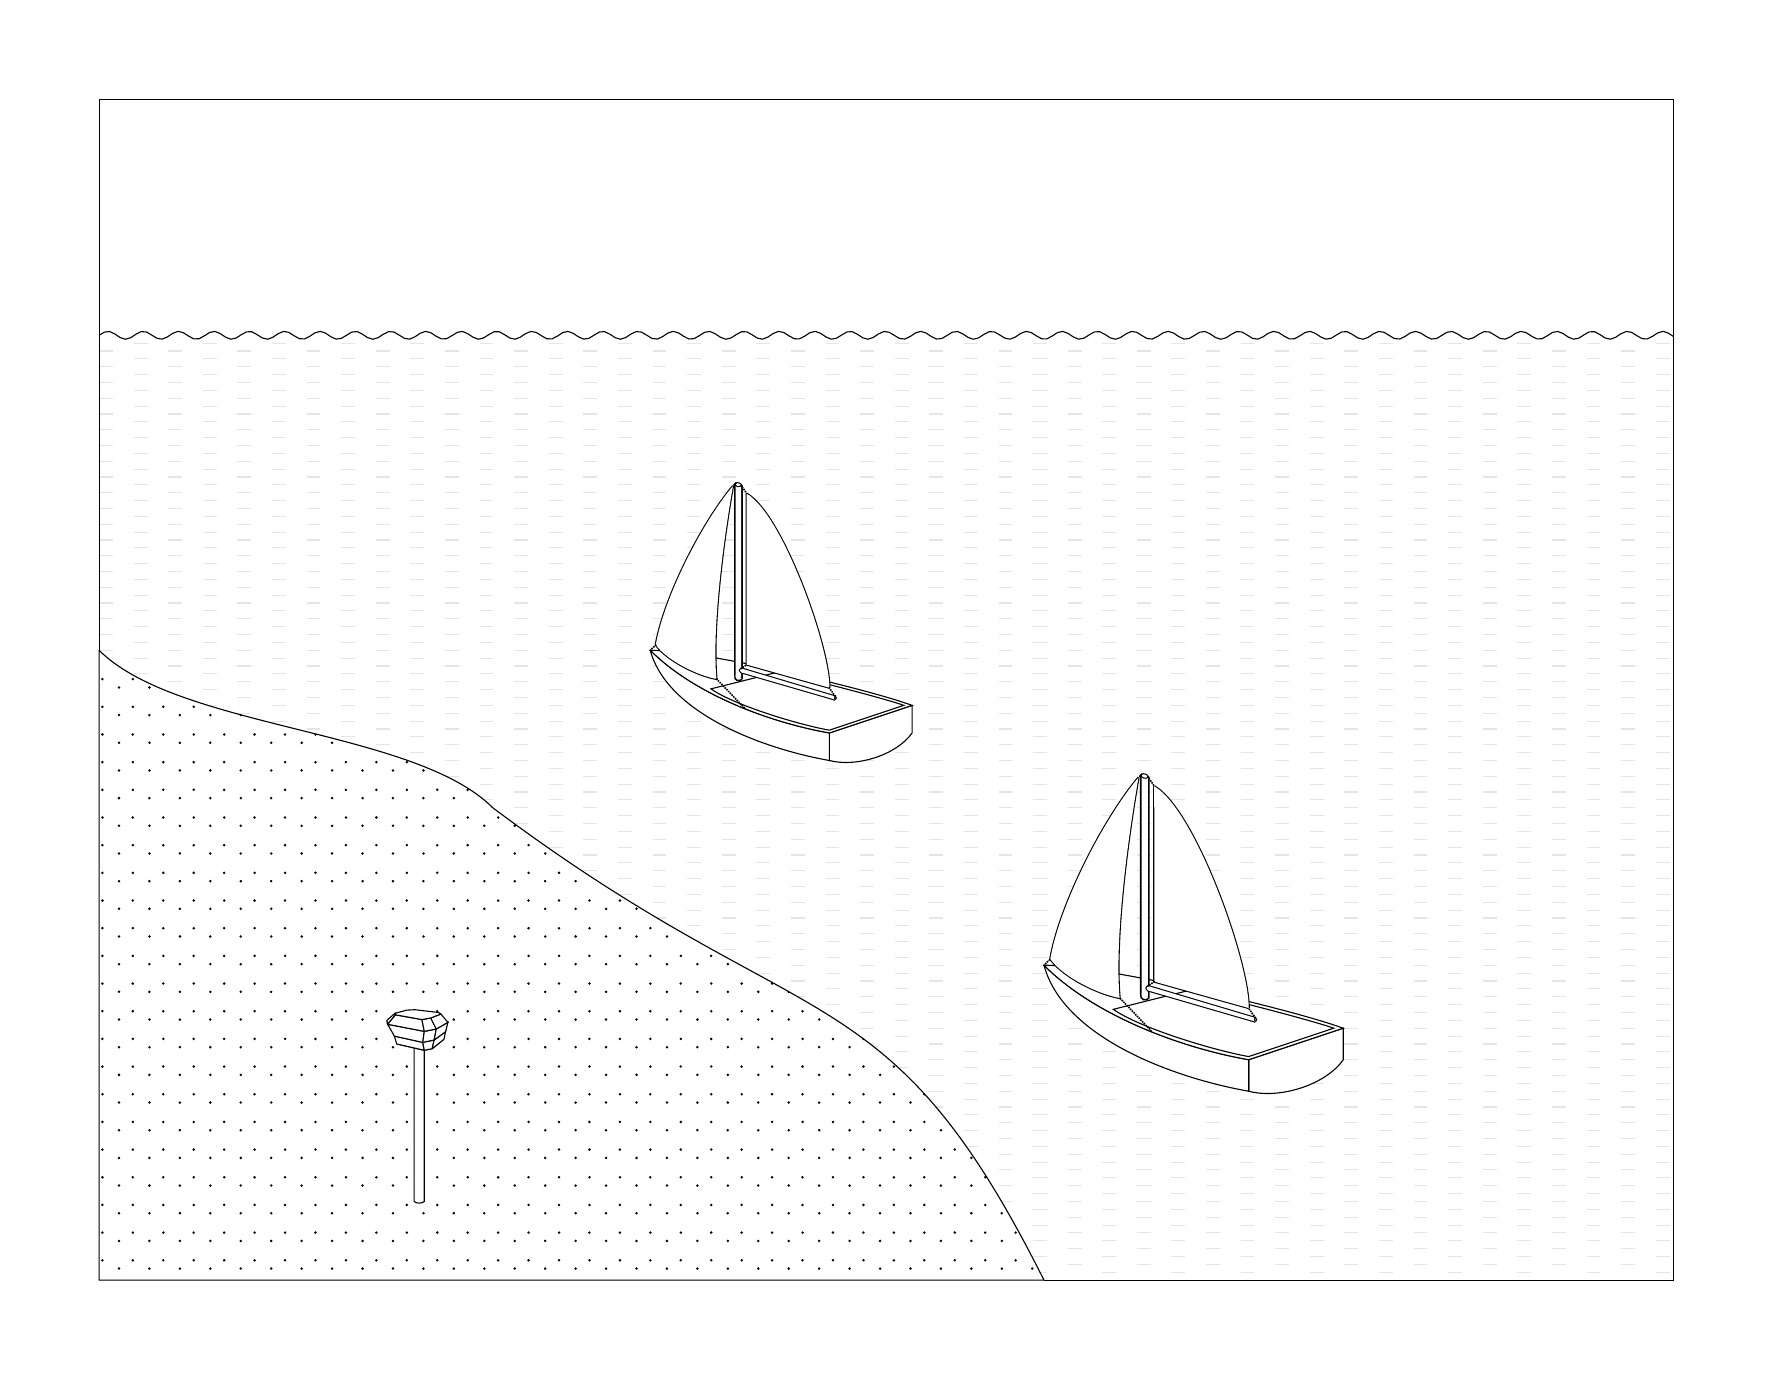
\begin{tikzpicture}[domain=0:20,samples=300]
  \begin{pgfonlayer}{foreground}
    % \draw[step=1cm,black,thin,opacity=0.2,dashed] (20.9,-0.9) grid (-0.9,15.9);
    \draw[opacity=0] (20.9,-0.9) grid (-0.9,15.9);
  
    \draw (0,8) -- (0,15) -- (20,15) -- (20,0) -- (12,0);
  
    \draw[fill=white,draw opacity=0] 
      (0,8) -- (0,0) -- (12,0) .. controls (10,4) and (9,3) .. (5,6) .. controls (4,7) and (1,7) .. (0,8);
    \draw[pattern=my crosshatch dots] 
      (0,8) -- (0,0) -- (12,0) .. controls (10,4) and (9,3) .. (5,6) .. controls (4,7) and (1,7) .. (0,8);
  
    \draw plot(\x,{sin(14 * \x r) / 20 + 12});
  
    \path (12,4) pic[scale=0.8] {boat};
    \path (7,8) pic[scale=0.7] {boat};
    
    % Receiver
    \coordinate (pole_left_bottom) at (4,1);
    \coordinate (pole_right_bottom) at (4.13,1);
    \coordinate (pole_left_top) at ($ (pole_left_bottom) + (0,2) $);
    \coordinate (pole_right_top) at ($ (pole_right_bottom) + (0,2) $);
    
    \draw[fill=white]
      (pole_left_top)
      --
      (pole_left_bottom)
      to[out=-45,in=-135,looseness=0.8]
      (pole_right_bottom)
      --
      (pole_right_top);
      
    \coordinate (rs_core_1) at ($ (pole_left_top) + (-0.22,0) $);
    \coordinate (rs_core_2) at ($ (rs_core_1) + (0.35,-0.08) $);
    \coordinate (rs_core_3) at ($ (rs_core_2) + (0.1,0.02) $);
    \coordinate (rs_core_4) at ($ (rs_core_3) + (0.15,0.12) $);
    \coordinate (rs_side_1) at ($ (rs_core_1) + (-0.03,0.1) $);
    \coordinate (rs_side_2) at ($ (rs_core_2) + (-0.02,0.1) $);
    \coordinate (rs_side_3) at ($ (rs_core_3) + (0.025,0.11) $);
    \coordinate (rs_side_4) at ($ (rs_core_4) + (0.02,0.095) $);
    \coordinate (rs_upper_1) at ($ (rs_side_1) + (-0.085,0.15) $);
    \coordinate (rs_upper_0) at ($ (rs_upper_1) + (-0.01,0.05) $);
    \coordinate (rs_upper_2) at ($ (rs_side_2) + (0.02,0.14) $);
    \coordinate (rs_upper_3) at ($ (rs_side_3) + (0.027,0.14) $);
    \coordinate (rs_upper_4) at ($ (rs_side_4) + (0.03,0.12) $);
    \coordinate (rs_top_1) at ($ (rs_upper_1) + (0.1,0.12) $);
    \coordinate (rs_top_0) at ($ (rs_top_1) + (-0.007,0.02) $);
    \coordinate (rs_top_2) at ($ (rs_upper_2) + (-0.03,0.15) $);
    \coordinate (rs_top_3) at ($ (rs_upper_3) + (-0.07,0.14) $);
    \coordinate (rs_top_4) at ($ (rs_upper_4) + (-0.09,0.105) $);
    \coordinate (rs_top_5) at ($ (rs_top_4) + (-0.03,0.02) $);
    \coordinate (rs_top_6) at ($ (rs_top_5) + (-0.3,0.035) $);
    \coordinate (rs_top_7) at ($ (rs_top_6) + (-0.1,-0.005) $);
    
    \draw[fill=white]
      (rs_core_1) -- (rs_core_2) -- (rs_core_3) -- (rs_core_4);
      
    \draw[fill=white]
      (rs_core_1) -- (rs_side_1) -- (rs_side_2) -- (rs_core_2) -- (rs_core_1);
      
    \draw[fill=white]
      (rs_core_2) -- (rs_side_2) -- (rs_side_3) -- (rs_core_3) -- (rs_core_2);
      
    \draw[fill=white]
      (rs_core_3) -- (rs_side_3) -- (rs_side_4) -- (rs_core_4) -- (rs_core_3);
      
    \draw[fill=white]
      (rs_side_1) -- (rs_upper_1) -- (rs_upper_2) -- (rs_side_2) -- (rs_side_1);
      
    \draw[fill=white]
      (rs_side_2) -- (rs_upper_2) -- (rs_upper_3) -- (rs_side_3) -- (rs_side_2);
      
    \draw[fill=white]
      (rs_side_3) -- (rs_upper_3) -- (rs_upper_4) -- (rs_side_4) -- (rs_side_3);
      
    \draw
      (rs_upper_1) -- (rs_upper_0);
      
    \draw[fill=white]
      (rs_upper_0) -- (rs_top_0) -- (rs_top_1) -- (rs_upper_1) -- (rs_upper_0);
    
    \draw[fill=white]
      (rs_upper_1) -- (rs_top_1) -- (rs_top_2) -- (rs_upper_2) -- (rs_upper_1);
      
    \draw[fill=white]
      (rs_upper_2) -- (rs_top_2) -- (rs_top_3) -- (rs_upper_3) -- (rs_upper_2);
      
    \draw[fill=white]
      (rs_upper_3) -- (rs_top_3) -- (rs_top_4) -- (rs_upper_4) -- (rs_upper_3);
      
    \draw[fill=white]
      (rs_top_0) -- (rs_top_1) -- (rs_top_2) -- (rs_top_3) -- (rs_top_4) --
      (rs_top_5) -- (rs_top_6) -- (rs_top_7) -- (rs_top_0);
  \end{pgfonlayer}
  
  \begin{pgfonlayer}{background}
    \foreach \x in {11.9,11.7,...,0.1}{
      \draw[gray!20,dash pattern=on 5pt off 20pt] ([xshift=12.5pt]0cm, \x cm) -- ++([xshift=-12.5pt]20cm, 0);
    }
    \foreach \x in {11.8,11.6,...,0.2}{
      \draw[gray!20,dash pattern=on 5pt off 20pt] (0cm, \x cm) -- ++(20cm, 0);
    }
  \end{pgfonlayer}
\end{tikzpicture}
\end{document}